\documentclass[conference]{IEEEtran}
\usepackage[T1]{fontenc}
\usepackage[utf8]{inputenc}
\usepackage{amsmath,amssymb}
\usepackage{graphicx}
\usepackage{booktabs}
\usepackage{cite}
\usepackage{url}

\newcommand{\tabref}[1]{Table~\ref{#1}}
\newcommand{\figref}[1]{Fig.~\ref{#1}}
\newcommand{\secref}[1]{Section~\ref{#1}}
\newcommand{\Ldec}{\mathcal{L}_\mathrm{mix}^\mathrm{dec}}
\newcommand{\Lenc}{\mathcal{L}_\mathrm{mix}^\mathrm{enc}}

\begin{document}

\title{Latent Arithmetic Measures the Origin:\\A No-Retraining Intervention on Audio Autoencoders}

\author{\IEEEauthorblockN{Nurdaulet Akhanov}
\IEEEauthorblockA{Mohamed bin Zayed University of Artificial Intelligence\\
Abu Dhabi, United Arab Emirates\\
nurdaulet.akhanov@mbzuai.ac.ae}}

\maketitle

\begin{abstract}
Audio latents are increasingly evaluated by arithmetic: interpolate two codes
and decode a mix, subtract a stem's code and decode the residual. We show that
one of these two probes is not a property of the autoencoder at all. Shifting
the latent origin by the encoded silence $f(0)$, a reparameterization that
leaves the autoencoding function and every affine combination with unit
coefficient sum exactly unchanged for arbitrary nonlinear encoders and
decoders, changes stem-subtraction scores by several decibels. Applying it to
five fixed checkpoints, with no retraining, removes the entire apparent
advantage of mixing supervision on subtraction: an advantage of $+2.3$ to
$+4.0$\,dB becomes $-0.07$ to $+0.01$\,dB, a reduction on all 49 test tracks,
and every model lands within $0.5$\,dB of its own reconstruction of the
residual. On convex mixing, which the same reparameterization provably cannot
touch, the supervision does help: ground-truth equivariance improves by
$+1.7$ to $+2.2$\,dB at two compression rates. The two probes therefore
support different conclusions about the same checkpoints, and latent
arithmetic should be reported against a coordinate-invariant reference.
\end{abstract}

\begin{IEEEkeywords}
representation learning, equivariant representations, audio autoencoders, latent arithmetic, evaluation methodology, source separation
\end{IEEEkeywords}

\section{Introduction}\label{sec:intro}
Audio mixing is linear on waveforms:
$\mathrm{mix}(x_1,x_2,\alpha)=\alpha x_1+(1{-}\alpha)x_2$. This makes latent
arithmetic an attractive interface to a learned audio representation. For an
encoder $f$ and decoder $g$, a latent space is \emph{mixing-equivariant} when
\begin{equation}
  g\!\left(\alpha f(x_1)+(1{-}\alpha)f(x_2)\right)\approx \alpha x_1+(1{-}\alpha)x_2 ,
  \label{eq:equiv}
\end{equation}
and a natural companion probe is stem removal by subtraction,
$g(f(x_\mathrm{mix}){-}f(x_\mathrm{stem}))\approx x_\mathrm{res}$. Where these
hold, editing and composition happen in the latent domain without a
dedicated separation or synthesis model, a prerequisite for latent-diffusion
systems \cite{liu2023audioldm,evans2024stable} that compose independently
modeled sources. Standard autoencoders do not satisfy Eq.~\ref{eq:equiv}:
their objectives reward reconstruction fidelity, not algebraic structure, and
in quantized codecs (DAC \cite{kumar2024dac}, EnCodec
\cite{defossez2023encodec}) an interpolated point is not a codebook entry,
so code-domain mixing is undefined without leaving the quantizer. Torres et al.~\cite{torres2026linearity} induce the property in a
consistency autoencoder by decoding averaged latents against the true mix.

This paper asks a prior question: \emph{what do these arithmetic scores
measure?} The two probes differ in one respect that is easy to overlook. The
coefficients in Eq.~\ref{eq:equiv} sum to one; those of subtraction sum to
zero. Latents are defined only up to a choice of origin, and a shift of that
origin cancels in the first case but not in the second. \secref{sec:origin}
makes this precise for arbitrary nonlinear $f$ and $g$: recentering the latent
space at $f(0)$ leaves the autoencoding function and every unit-sum
combination pointwise identical, while mapping subtraction to
$g(f(x_\mathrm{mix}){-}f(x_\mathrm{stem}){+}f(0))$. Any change a subtraction
score shows under this map is therefore a property of the coordinate system,
not of the model as a function.

We run that intervention on five fixed checkpoints of a waveform GAN
autoencoder, spanning two compression rates and three training objectives,
with no retraining and no change to the evaluation audio. Our contributions:
\begin{enumerate}
  \item A reparameterization argument (\secref{sec:origin}) showing that
  subtraction-style latent arithmetic is coordinate-dependent while
  reconstruction and convex mixing are not, and identifying the model's own
  reconstruction of the target as the coordinate-invariant reference.
  \item The intervention applied to fixed checkpoints
  (\secref{sec:subtraction}): recentering removes the entire aggregate
  advantage that mixing supervision appears to have on stem subtraction,
  on every one of the 49 test tracks, while small stem-dependent differences
  survive.
  \item Evidence that the two probes disagree on the same checkpoints
  (\secref{sec:mixing}): on convex mixing, which the intervention cannot
  affect, the supervision does deliver a measurable gain at both compression
  rates, and it also restores level, not only spectral shape.
  \item A methodological correction (\secref{sec:protocol}): the widely used
decode-vs-decode SI-SDR is inflated by an adversarial term and by decoder
sampling noise; we report a ground-truth-referenced variant.
\end{enumerate}

\section{Related Work}\label{sec:related}
\textbf{Neural audio codecs.} DAC \cite{kumar2024dac},
EnCodec \cite{defossez2023encodec} and SoundStream \cite{zeghidour2022soundstream}
pair convolutional encoders with HiFi-GAN decoders \cite{kong2020hifigan} and
multi-scale discriminators, optimizing reconstruction without latent
structure; their residual vector quantization also precludes latent
interpolation. RAVE \cite{caillon2021rave} learns a variational latent space
but does not target mixing equivariance, and disentanglement regularizers
\cite{higgins2017betavae} encourage generic smoothness rather than a specific
algebraic identity.
Mixing-equivariance follows the symmetry-based view of representation
learning \cite{higgins2018towards}, though convex mixing is an affine
combination, not a group action. \textbf{Linear audio representations.} Music2Latent
\cite{pasini2024music2latent} is a consistency autoencoder with partial
linearity as a byproduct. Torres et al.~\cite{torres2026linearity} make it
approximately linear by conditioning the decoder on the average of separately
encoded latents while denoising the true mix under the unchanged consistency
loss, a principle related to mixup \cite{zhang2018mixup}. Their additivity
and separation scores compare two decodes, a protocol \secref{sec:protocol}
shows to be confounded, and their separation is negative on every stem
($-0.3$ to $-1.8$\,dB). No prior work reports latent arithmetic against a
declared origin.

\section{The Latent Origin Is a Free Coordinate}\label{sec:origin}

\noindent\textbf{Proposition.} Let $f:\mathcal{X}\to\mathcal{Z}$ and
$g:\mathcal{Z}\to\mathcal{X}$ be arbitrary maps, and define the recentered
pair
\begin{equation}
  f_c(x)=f(x)-f(0), \qquad g_c(z)=g\!\left(z+f(0)\right).
  \label{eq:recenter}
\end{equation}
Then (i) $g_c(f_c(x))=g(f(x))$ for every $x$; (ii) for any $x_1,\dots,x_n$ and
any coefficients with $\sum_i\alpha_i=1$,
$g_c\!\left(\sum_i\alpha_i f_c(x_i)\right)=g\!\left(\sum_i\alpha_i f(x_i)\right)$;
and (iii) for the coefficients $(1,-1)$,
\begin{equation}
  g_c\!\left(f_c(x)-f_c(y)\right)=g\!\left(f(x)-f(y)+f(0)\right).
  \label{eq:sub}
\end{equation}

\noindent\emph{Proof.} $f_c(x)+f(0)=f(x)$ gives (i). For (ii),
$\sum_i\alpha_i f_c(x_i)=\sum_i\alpha_i f(x_i)-f(0)\sum_i\alpha_i
=\sum_i\alpha_i f(x_i)-f(0)$, and $g_c$ adds $f(0)$ back. For (iii) the
coefficients sum to zero, so the offset cancels in the latent difference,
$f_c(x)-f_c(y)=f(x)-f(y)$, and $g_c$ adds $f(0)$ inside $g$. $\square$

Three consequences shape the rest of the paper. First, $(f_c,g_c)$ is
\emph{the same autoencoder} as $(f,g)$ as far as reconstruction and
Eq.~\ref{eq:equiv} are concerned: by (i) and (ii) those quantities are
pointwise identical, for arbitrary nonlinear networks, with no retraining and
no approximation. Second, by (iii) subtraction is not: recentering shifts it
by one encode of silence, and \secref{sec:subtraction} measures a several-decibel
shift. A model ranking obtained from raw subtraction can therefore be altered
by a change of coordinates that provably leaves reconstruction and mixing
untouched, so such a ranking is not by itself a statement about the
representation. Third, when $f$ happens to be affine, $f(x)=Ax+b$, we have
$f(x){-}f(y){+}f(0)=f(x{-}y)$ and Eq.~\ref{eq:sub} decodes exactly
$g(f(x_\mathrm{res}))$: the model's own reconstruction of the residual,
whatever the decoder does. That quantity, the encode--decode reconstruction of
the target, is the reference we report against; the shortfall from it is the
\emph{linearity tax}. How far a real encoder departs from affine is empirical,
so the recovery is exact only in the affine limit and approximate here.

\section{Experimental Setup}\label{sec:setup}

\subsection{Models and supervision}\label{sec:models}
The primary model is a waveform autoencoder (DAC-style 1-D convolutional
encoder, HiFi-GAN decoder \cite{kong2020hifigan}, combined multi-scale-STFT
and multi-period discriminator) at 44.1\,kHz on 1-second mono chunks, trained
on a ${\sim}$950-hour union of FMA-large, MAESTRO and MUSDB18-HQ
\cite{rafii2017musdb18}.\footnote{Code, training configurations, pretrained
weights, every metric reported here, and audio examples:
\url{https://github.com/nurdauletakhanov/musicgen}} Two compression regimes
are used: $7.66\times$ ($d{=}128$) and $15.3\times$ ($d{=}64$).

Mixing supervision is the explicit-loss form of the additivity principle of
\cite{torres2026linearity}. We form pairs $(x_i,x_j)$ with a fixed-point-free permutation and draw
$\alpha\sim U[0,1]$; with
$\bar{x}=\alpha x_i{+}(1{-}\alpha)x_j$ and
$\bar{z}=\alpha f(x_i){+}(1{-}\alpha)f(x_j)$, the decode-mixing loss is, as
implemented,
\begin{equation}
  \Ldec=\mathcal{L}_\mathrm{recon}\!\left(g(\bar{z}),\bar{x}\right)
        +\lVert g(\bar{z})-\bar{x}\rVert_1 ,
  \label{eq:ldec}
\end{equation}
where $\mathcal{L}_\mathrm{recon}$ is the weighted multi-resolution STFT and
mel loss also used for reconstruction; the mixed path carries the extra
unweighted waveform $\ell_1$ term, the ordinary reconstruction path does not.
Gradients flow through $g$ and into $f$ via $\bar{z}$. The total objective
is
$\mathcal{L}=\mathcal{L}_\mathrm{recon}+\mathcal{L}_\mathrm{GAN}+\lambda\Ldec
+\lambda_{\ell_2}\lVert z\rVert^2$; a variant additionally applies the
discriminator to the mixed path (``$+$disc''). Mixing losses are added either
as a 25k-step fine-tune over a converged baseline ($7.66\times$) or from
scratch over 250k steps ($15.3\times$), each against a matched control that is
identical except that mixing is disabled. All runs use a single NVIDIA
RTX~5090.

\subsection{Metrics}\label{sec:metrics}
We report reconstruction SI-SDR$_\mathrm{rec}=\mathrm{SISDR}(g(f(x)),x)$ and,
at $\alpha{=}0.5$, two equivariance views:
SI-SDR$_\mathrm{lin}=\mathrm{SISDR}(g(\bar{z}),g(f(\bar{x})))$
(decode-vs-decode, relative to the model's own reconstruction of the mix) and
SI-SDR$_\mathrm{lin}^\mathrm{gt}=\mathrm{SISDR}(g(\bar{z}),\bar{x})$ (vs.\
ground truth, the quantity in Eq.~\ref{eq:equiv} up to scale and comparable
across models). We also report
$\ell_\mathrm{lat}=\lVert\bar{z}-f(\bar{x})\rVert^2/\lVert f(\bar{x})\rVert^2$
and MixRate $=\mathcal{L}_\mathrm{mix}(g(\bar{z}),\bar{x})/
\mathcal{L}_\mathrm{mix}(g(f(\bar{x})),\bar{x})$, with
$\mathcal{L}_\mathrm{mix}$ the three-term mixed-path loss of
Eq.~\ref{eq:ldec} in both numerator and denominator ($<1$ beats the
encode-then-decode path). SI-SDR$_\mathrm{lin}$ shares the decode-vs-decode
structure of prior additivity metrics \cite{torres2026linearity} and can be moved without ground-truth equivariance moving
(\secref{sec:mixing}); SI-SDR$_\mathrm{lin}^\mathrm{gt}$ and MixRate are our
metrics of record. SI-SDR fits a gain before scoring, so it does not
assess level preservation; we report the fitted gain separately.

\subsection{Protocol and what the intervals cover}\label{sec:protocol-setup}
Subtraction is evaluated on the MUSDB18 test set, 49 of 50 tracks (one is
excluded because its stems sum to the mixture at only $18.5$\,dB), giving
5{,}880 (track, stem, chunk) units; chunk selection is a pure function of the
seed and the sorted track list, so all models are measured on identical units
and every contrast is paired. Confidence intervals come from a paired cluster
bootstrap over the 49 tracks ($10^4$ resamples), the correlated unit. They are
a \emph{conditional diagnostic}: they cover evaluation variance over test
audio for these checkpoints, and cover neither training-seed variance nor
checkpoint selection.

That selection needs disclosure. The released weights are the checkpoint with
the lowest validation loss, and the validation loader read the test split. For
every $7.66\times$ run this coincides with the final step, so selection did
not alter those weights; both $15.3\times$ runs were selected at step 240k of
250k. Contrasts are between matched configurations under identical selection,
and the origin intervention is applied to fixed checkpoints so it is unaffected,
but absolute generalization claims should be read with this in mind. The code
now supports a held-out validation split.

\section{Results}\label{sec:results}

\subsection{Recentering removes the subtraction advantage}\label{sec:subtraction}
We remove a stem by latent subtraction,
$\hat{x}=g(f(x_\mathrm{mix}){-}f(x_\mathrm{stem}))$, and score SI-SDR against
the true residual. This is an \emph{oracle} setting: the removed stem is
available and encoded, so it probes the representation's arithmetic, not blind
separation; its use is latent-domain editing when stem codes exist. The
intervention of
\secref{sec:origin} replaces this by
$g(f(x_\mathrm{mix}){-}f(x_\mathrm{stem}){+}f(0))$, which by
Eq.~\ref{eq:sub} is the same model read in recentered coordinates.

\begin{table}[t]
  \centering\small
  \setlength{\tabcolsep}{2.2pt}
  % AUTO-GENERATED by make_tables.py — do not edit by hand (regenerate via make_tables.py).
\begin{tabular}{@{}lcccccc@{}}
\toprule
Model & drums & bass & vocals & other & all & gap$\downarrow$ \\
\midrule
    7.66$\times$ no mix & +4.2 & +0.4 & +5.2 & +3.9 & +3.4 & 5.2 \\
    \quad $+f(0)$ & +8.8 & +6.8 & +9.6 & +8.0 & +8.3 & 0.4 \\
    7.66$\times$ $+\mathcal{L}_\mathrm{dec}$ & +5.7 & +4.9 & +7.2 & +5.1 & +5.7 & 3.0 \\
    \quad $+f(0)$ & +8.5 & +6.9 & +9.4 & +8.3 & +8.3 & 0.5 \\
    7.66$\times$ $+\mathcal{L}_\mathrm{dec}$+disc & +6.2 & +5.4 & +7.5 & +5.0 & +6.0 & 2.6 \\
    \quad $+f(0)$ & +8.5 & +7.0 & +9.3 & +8.1 & +8.2 & 0.4 \\
    \midrule
    15.3$\times$ no mix & +1.2 & -1.6 & +3.0 & +2.1 & +1.2 & 6.6 \\
    \quad $+f(0)$ & +7.3 & +5.8 & +8.8 & +7.2 & +7.3 & 0.5 \\
    15.3$\times$ +mix & +5.4 & +4.7 & +6.9 & +3.9 & +5.2 & 2.5 \\
    \quad $+f(0)$ & +7.3 & +6.1 & +8.5 & +7.2 & +7.3 & 0.4 \\
    \midrule
    M2L +mix & -9.9 & -12.3 & -9.9 & -12.7 & -11.2 & 8.4 \\
\bottomrule
\end{tabular}

  \caption{Stem removal by latent subtraction (SI-SDR, dB; MUSDB18 test,
  5{,}880 units from 49 tracks). ``$+f(0)$'' rows read the \emph{same}
  checkpoint in recentered coordinates. ``gap'' is the linearity tax against
  each model's own encode--decode reconstruction of the residual (lower is
  better).}
  \label{tab:subtraction}
\end{table}

\begin{table}[t]
  \centering\small
  \setlength{\tabcolsep}{3.0pt}
  % AUTO-GENERATED by make_tables.py — do not edit by hand (regenerate via make_tables.py).
\begin{tabular}{@{}lccrc@{}}
\toprule
Treatment vs.\ its control & raw & recent. & 95\% CI & tracks \\
\midrule
    \multicolumn{5}{@{}l}{\emph{MUSDB18 test (49 tracks)}} \\
    \quad $\Ldec$, 7.66$\times$ & +2.33 & -0.03 & [-0.15, +0.10] & 49/49 \\
    \quad $\Ldec{+}$disc, 7.66$\times$ & +2.64 & -0.07 & [-0.19, +0.07] & 49/49 \\
    \quad $\Ldec{+}$disc, 15.3$\times$ & +4.02 & +0.01 & [-0.19, +0.21] & 49/49 \\
    \midrule
    \multicolumn{5}{@{}l}{\emph{MoisesDB, held out (240 tracks)}} \\
    \quad $\Ldec$, 7.66$\times$ & +2.27 & +0.29 & [+0.20, +0.39] & 240/240 \\
    \quad $\Ldec{+}$disc, 7.66$\times$ & +2.47 & +0.12 & [+0.03, +0.22] & 240/240 \\
    \quad $\Ldec{+}$disc, 15.3$\times$ & +4.50 & +0.42 & [+0.29, +0.55] & 240/240 \\
\bottomrule
\end{tabular}

  \caption{The intervention on fixed checkpoints. Advantage in stem-subtraction SI-SDR (dB) of each mixing-trained model over the matched control at the same compression rate trained without
  mixing supervision, before and after recentering,
with the paired change and the number of tracks on which the advantage
shrinks. Recentering is a change of coordinates only: no retraining, same
units, same audio.}
  \label{tab:origin}
\end{table}

\textbf{In raw coordinates the supervision looks decisive.} Mixing
supervision raises subtraction quality from $+3.4$ to $+5.8$\,dB at
$7.66\times$ and from $+1.2$ to $+5.2$\,dB at $15.3\times$
(\tabref{tab:subtraction}), advantages of $+2.33$ and $+4.02$\,dB on paired
units (\tabref{tab:origin}).

\textbf{Recentering erases it.} Adding $f(0)$ gains $+2.0$ to $+6.0$\,dB for
every evaluated configuration and leaves each within $0.4$--$0.5$\,dB of its
own reconstruction reference in aggregate; the models that gain most are the
ones that looked worst. The between-model advantage falls to $-0.03$,
$-0.07$ and $+0.01$\,dB, all three intervals containing zero
(\tabref{tab:origin}), and the reduction holds on $49$ of $49$ tracks in every
pair (\figref{fig:origin}, right). The no-mixing models also carry the larger
offset ($\lVert f(0)\rVert$ $6.6$ versus $5.4$ at $7.66\times$, $18.1$ versus
$14.8$ at $15.3\times$), though offset norm alone does not determine the
decoded error, which also depends on latent scale and decoder sensitivity.

\begin{figure*}[t]
  \centering
  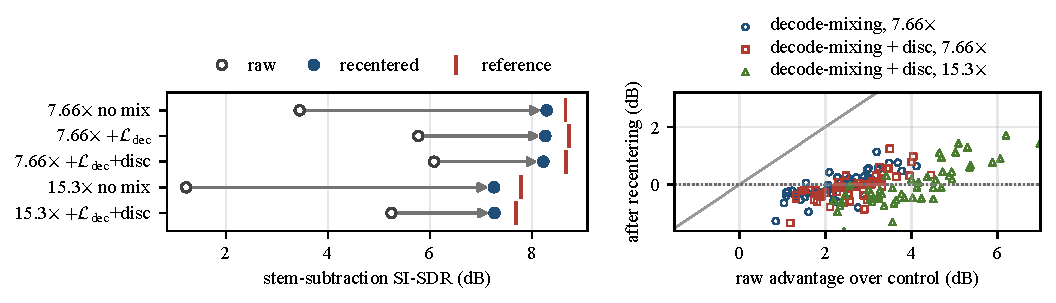
\includegraphics[width=\textwidth]{figures/fig_origin.pdf}
  \caption{The origin intervention on five fixed checkpoints. \emph{Left:}
  stem-subtraction SI-SDR moves from raw coordinates to recentered ones
  (arrow), landing at each model's own reconstruction of the residual (red
  tick); the raw ordering does not survive. \emph{Right:} per-track advantage
  over the matched no-mixing control, raw (horizontal) against recentered
  (vertical), one point per track. Every point falls below the diagonal and
  the recentered values sit at zero.}
  \label{fig:origin}
\end{figure*}

\textbf{What survives.} Recentering equalizes the aggregate, not everything.
Per stem the recentered contrast is still nonzero in both directions: at
$15.3\times$, $+0.35$\,dB on bass and $-0.34$\,dB on vocals; at $7.66\times$,
$+0.37$ on ``other'' against $-0.31$ on drums. Mixing supervision moves where
the arithmetic error sits across sources without moving its mean. The
residual $0.4$--$0.5$\,dB gap to the reference is what decoding leaves after
recentering, not a direct measure of encoder non-affinity; per track the tail
is wider (worst $2.2$\,dB, $29$--$32$ of $49$ tracks within $0.5$\,dB).

\textbf{Baselines without latent arithmetic.} The unchanged mixture scores
$+17.1$\,dB against the residual, above every model's reconstruction
reference, because the removed stem is a small share of the energy: the
metric certifies arithmetic only relative to the model's own reconstruction.
Autoencoding the mixture unchanged scores $+2.2$\,dB ($+1.7$ at
$15.3\times$), decoding both signals and subtracting waveforms $+7.5$
($+6.5$). Recentered latent subtraction beats waveform subtraction by $+0.7$
to $+0.9$\,dB (intervals exclude zero), raw subtraction loses to it
everywhere.

\subsection{Convex mixing tells a different story}\label{sec:mixing}
By part (ii) of the proposition, recentering cannot change any quantity in
Eq.~\ref{eq:equiv}. The mixing probe therefore reports on the autoencoder
itself, and there the supervision does something (\tabref{tab:crossarch}). At
$7.66\times$, $\Ldec$ improves ground-truth equivariance from $8.0$ to $10.2$\,dB and is
the only configuration with MixRate $<1$; reconstruction SI-SDR spans
$11.2$--$11.4$\,dB and FAD $0.044$--$0.046$, so we observe no reconstruction
cost at this rate, on single runs that cannot establish the absence of a
difference this small. Trained from
scratch at $15.3\times$ against a matched control, the combined
$\Ldec{+}$disc recipe improves SI-SDR$_\mathrm{lin}^\mathrm{gt}$ from $6.8$
to $8.6$\,dB, MixRate from $1.19$ to $1.05$ and encoder linearity
$\ell_\mathrm{lat}$ from $0.078$ to $0.057$ at equal reconstruction
($9.9$ vs.\ $10.0$\,dB), while FAD rises from $0.052$ to $0.061$; whether that
is perceptible is untested. The $15.3\times$ pair differs by the whole
combined recipe, so it attributes the gain to that recipe against its control
and does not isolate the contribution of $\Ldec$ alone at that rate.

\begin{table}[t]
  \centering\small
  \setlength{\tabcolsep}{2.0pt}
  % AUTO-GENERATED by make_tables.py — do not edit by hand (regenerate via make_tables.py).
\begin{tabular}{@{}lccccc@{}}
\toprule
Model & SDR$_\mathrm{rec}$ & SDR$_\mathrm{lin}$ & SDR$_\mathrm{lin}^\mathrm{gt}$ & MixRate & FAD \\
\midrule
    GAN AE, 7.66$\times$, no mix & +11.3 & +12.0 & +8.0 & 1.203 & 0.045 \\
    GAN AE, 7.66$\times$, +mix & +11.4 & +12.1 & +10.2 & 0.972 & 0.044 \\
    GAN AE, 15.3$\times$, no mix & +10.0 & +10.6 & +6.8 & 1.187 & 0.052 \\
    GAN AE, 15.3$\times$, +mix & +9.9 & +14.6 & +8.6 & 1.046 & 0.061 \\
    M2L, no mix (baseline) & -3.3 & +5.0 & -9.6 & 1.101 & 0.127 \\
    M2L, fine-tune control & -3.1 & +5.1 & -9.5 & 1.125 & -- \\
    M2L, +mix & -2.6 & +6.9 & -7.8 & 1.086 & 0.119 \\
\bottomrule
\end{tabular}

  \caption{Convex mixing across compression and architecture (full test set,
  $\alpha{=}0.5$, EMA weights for Music2Latent). The M2L ``fine-tune control''
  is the continued-training baseline with mixing disabled. These quantities
  are invariant to the intervention of \secref{sec:origin}.}
  \label{tab:crossarch}
\end{table}

\textbf{Level, not only shape.} SI-SDR discards gain, so we also report the
gain it fits: the decoded mix is $1.6$\,dB too quiet without the loss and
$0.9$\,dB with it, against the model's own reconstruction level error of
$0.8$\,dB; at $15.3\times$, $1.8$ versus $1.0$ against $0.9$.

\textbf{The mixed-path discriminator buys the metric, not the property.} At
$7.66\times$, adding an adversarial term on the mixed path leaves ground-truth
equivariance unchanged ($10.2\!\to\!9.9$\,dB, MixRate $0.97\!\to\!1.05$) while
raising decode-vs-decode SI-SDR$_\mathrm{lin}$ from $12.1$ to $16.0$\,dB. The two decode paths move toward each other without either moving toward
$\bar{x}$, so the two metrics rank these configurations differently. We do
not identify the mechanism. Whether the discriminator has an effect
without $\Ldec$ is not tested here.

\textbf{Architecture.} Fine-tuning the published Music2Latent
\cite{pasini2024music2latent} consistency autoencoder with the decode-mixing
objective improves SI-SDR$_\mathrm{lin}^\mathrm{gt}$ against a continued-training control ($-9.5\!\to\!-7.8$\,dB) but stays far from usable waveform
arithmetic; its subtraction is unusable outright ($-11.2$\,dB,
\tabref{tab:subtraction}). The systems differ in encoder, loss family, compression and
training data as well as decoder class, so the contrast isolates none of
them: we report it as a limit on transfer, not an explanation.

\subsection{Decode-vs-decode scores are protocol-sensitive}\label{sec:protocol}
For stochastic decoders the decode-vs-decode metric is confounded a second
way. A consistency-model decoder \cite{pasini2024music2latent} draws fresh noise per call: decoding the \emph{same} latent twice is
deterministic under shared noise but scores $-1.8$\,dB under independent
noise, with no latent arithmetic at all. On identical pairs
(\figref{fig:protocol}) the same checkpoints score $-9.1$ and $-7.3$\,dB
when the two decodes draw independent noise and $+3.6$ and $+5.9$\,dB when
they share it: a $13$\,dB swing driven by the evaluation protocol rather
than the model. Which protocol prior work used is not stated in enough
detail for us to determine. We use shared decode noise
everywhere.

\begin{figure}[t]
  \centering
  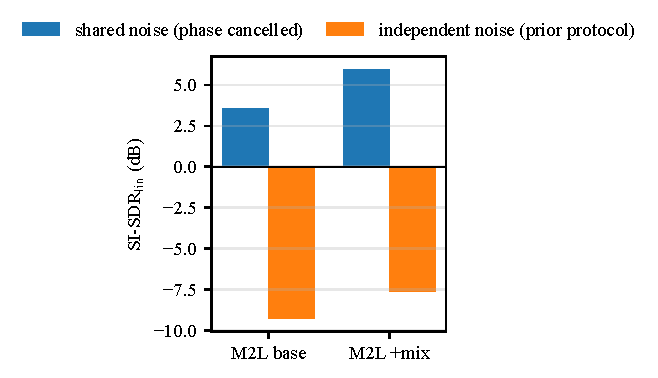
\includegraphics[scale=1]{figures/fig_protocol.pdf}
  \caption{Decode-noise protocol confound (Music2Latent, MUSDB18,
  $\alpha{=}0.5$). The same checkpoints score deeply negative under
  independent-noise decoding and positive under shared-noise decoding; the
  negative scores reflect decoder sampling noise rather than latent
linearity.}
  \label{fig:protocol}
\end{figure}

\section{Conclusion}\label{sec:conclusion}
Latent stem subtraction is measured in coordinates that the model never fixes.
Recentering the latent space at the encoded silence leaves the autoencoding
function and every unit-sum combination pointwise unchanged, for arbitrary
nonlinear encoders and decoders, yet it moves subtraction scores by several
decibels and, on five fixed checkpoints, removes the entire aggregate
advantage that mixing supervision appeared to have there, on all 49 test
tracks. What the supervision buys is convex equivariance, which the intervention
cannot affect and which improves at both rates. We therefore recommend reporting latent arithmetic against a declared origin
and against the model's own reconstruction of the target.
\textbf{Limitations.} Comparisons are single-run at one initialization;
checkpoint selection used the test split (\secref{sec:protocol-setup});
intervals are conditional on these checkpoints; recovery is exact only for
an affine encoder; audio is mono and untested by listeners.

\bibliographystyle{IEEEtran}
\bibliography{references}

\end{document}
